This chapter introduces background theory, in particular Kalman and
Particle filtering and the application of these techniques to the
problem of simultaneous localisation and mapping (SLAM). First a
notation that will be used throughout this document is introduced in
Section~\ref{sec:Notation}. Section~\ref{sec:Kalman} gives a brief
overview of Kalman filter and Extended Kalman (Section~\ref{sec:EKF}).
Particle filter is introduced in Section~\ref{sec:PF}. A comparison of
Particle filter vs EKF follows in Section~\ref{sec:PFvsEKF}. A brief
overview of Localisation is given in Section~\ref{sec:Localisation},
followed by an overview of SLAM in Section~\ref{sec:SLAM}. Finally a
problem of revisiting or ``loop closing'' is discussed in
Section~\ref{sec:back_loop}.


\section {Notation}
\label{sec:Notation}

The pose of the robot is represented by $\x{k}{}{a}$. Superscript $a$
indicates a reference frame, $k$ is a discrete time. A map of the
region $a$ at time $k$ is $\map{k}{}{a}$. In the case when we need to
differentiate between different particles, we add an extra superscript
$m$ to indicate a particle index $\x{k}{a}{m}$ and $\map{k}{a}{m}$. A
control input at time $k$ is $\U{k}$. An observation taken at time $k$
is $\z{k}$. Further notation will be introduced later on in this
thesis. \refTable{tab:notation} summarises most of the symbols used in
this thesis.



\SILENT{
This section describes the notation that will be used throughout the
rest of the document. We reserve letter $k$ to represent discrete
time, letter $t$ will represent continuous time. Letters $a$ and $b$
will be used to index map frames. Letter $m$ is used to represent
particle index, the $m$-th particle or belonging to the $m$-th
particle. Index $i$ is reserved for numbering elements of the finite
sets, that do not directly depend on time, for example the map is a
finite set of landmarks, that does not directly depend on time.

The discrete time index will be a subscript, for example \z{k}. The
element index $i$ will also be subscript, if both time and element
index are present, the time index will be followed by a comma followed
by the element index.

Map and particle indices will be superscripts, if both present, the
map index will be first, followed by a comma followed by the particle
index. For example \x{}{a}{m} means the $m$-th particle in the $a$-th
map. Table~\ref{tab:notation} describes variables we will be using in the
thesis and their meaning.
}

\begin{table}[ht]
\begin{tabular}{|l|l|}
\hline
%
\x{k}{a}{m} & pose of the $m$-th particle in the $a$-th map frame 
              at time $k$. \\
\Xall{k}{a}{m} & path of the $m$-th particle in the $a$-th map frame 
                 from time $0$ to time $k$. \\
%
\U{k}    & control input at time $k$.\\
\Uall{k}{a} & subset of all control inputs up to time $k$, that apply to the map frame $a$.\\
%
\z{k}    & observation at time $k$. \\ 
\Zall{k}{a} & subset of all observations up to time $k$, that apply to the map frame $a$. \\ 
%
\Teleport{k}    & teleportation at time $k$.\\
\TeleportAll{k}{a} & subset of all teleportations up to time $k$, that apply to the map frame $a$.\\
%
\map{k}{a}{m} & map of the $m$-th particle in the map frame $a$ at time $k$\\
\mape{a}{m}{i} & $i$-th map element from the $m$-th particle's map in 
                  the map frame $a$.\\
%
\s{k}{a}{m} & $m$-th particle in the SLAM particle filter at time $k$,
              in the map frame $a$.\\
\Sall{k}{}    & set of all particles in the SLAM particle filter at time $k$.\\
%
\tr{i}{a}{b} & transition vector from map frame $a$ to map frame $b$. \\
%
\Trall{a}{b} & a set of transition vectors from map frame $a$ to $b$.\\
%
%
\sample{a}{p(A)}& $a$ is a sample from the distribution $p(A)$.\\
\gpath{a}{b} & path from map $a$ to map $b$.\\
\hline

\end{tabular}
\caption{Notation used throughout the thesis.}
\label{tab:notation}
\end{table}


\section{Kalman Filter}
\label{sec:Kalman}
%A bit of history
R.E. Kalman published his famous paper describing a recursive solution
to the linear filtering problem in 1960 \cite{kalman60}. Since then
the Kalman filter has been the subject of extensive research and
application in various fields of science. It is used heavily in the
science of robotics for localisation and mapping purposes.  Kalman
filtering is used in this research. What follows in this section is a
brief introduction to Kalman filtering.

The Kalman filter addresses a general problem of estimating the state $
\x{k}{}{} \in \Rset^n$ of a discrete-time controlled process that is
governed by the linear stochastic difference equation
\begin{equation}
\x{k}{}{} = A_k \x{k-1}{}{} + B_k \U{k-1} + w_{k-1},
\label{eqn:kalman_process}
\end{equation}
where $A_k$ is a matrix that describes evolution of the state from
time $k-1$ to $k$ in the absence of control input or process
noise, matrix $B_k$ relates control input $\U{k-1} \in \Rset^l$, to
the change in the state vector and $w_k$ is a process noise.

Indirect measurement of the state $\z{} \in \Rset^m$ is of the form
\begin{equation}
\z{k} = H_k \x{k}{}{} + v_k,
\label{eqn:kalman_obs}
\end{equation}
where $H_k$ is a matrix that relates the state to the observation at
time $k$, and $v_k$ is a measurement noise. Both process and
measurement noise are assumed to be zero mean Gaussian with known
covariances $Q_k$ and $R_k$ respectively. Process and measurement
noise are assumed to be independent of each other.

\begin{eqnarray}
w_k \sample{}{} N(0,Q_k),\\
v_k \sample{}{} N(0,R_k).
\end{eqnarray}


The true state of the system is not known, but an estimate of the
state at time $k$, $\hat{\x{}{}{}}_k$, can be computed recursively, if
the estimate of the initial state of the system is available. The
uncertainty of the estimate isassumed to be  Gaussian with the covariance
$\Sigma_k$.

The Kalman filter consists of two stages: time update and measurement
update. In the time update stage the filter predicts a new state,
based on the current state estimate and the process model. The
measurement update stage corrects the estimate using the new
measurement. For a good description of the derivation of the algorithm
see \cite{kalman_intro}. For the purposes of this document definition
of the filter update equations is sufficient.


\begin{eqnarray}
\label{eqn:kalman_x_u}
\hat{\x{}{}{}}_k^\prime &=& A_k \hat{\x{}{}{}}_{k-1} + B_k \U{k-1}\\
\label{eqn:kalman_sigma_u}
\Sigma_k^\prime &=& A_k \Sigma_{k-1} A_k^T + Q_{k-1}
\end{eqnarray}

Equations \refEquation{eqn:kalman_x_u} and
\refEquation{eqn:kalman_sigma_u}, constitute the prediction stage of the
Kalman filter. $\hat{\x{}{}{}}_k^\prime$ is a tentative estimate of
the state at time $k$, before incorporating the measurement,
$\Sigma_k^\prime$ is a covariance of the uncertainty of the tentative
estimate.

Measurement update equations are listed below:

\begin{eqnarray}
\label{eqn:kalman_gain}
K_k &=& \Sigma_k^\prime H_k^T (H_k \Sigma_k^\prime H_k^T + R_k )^{-1}\\
\label{eqn:kalman_x_obs}
\hat{\x{}{}{}}_k &=& \hat{\x{}{}{}}_k^\prime + 
                      K_k (\z{k} - H_k \hat{\x{}{}{}}_k^\prime)\\
\label{eqn:kalman_sigma_obs}
\Sigma_k &=& (I - K_k H_k) \Sigma_k^\prime
\end{eqnarray}

Equation \refEquation{eqn:kalman_gain} computes the Kalman gain,
$K_k$. The Kalman gain defines the contribution of the observation to
the new state estimate. $K_k$ is then used in
\refEquation{eqn:kalman_x_obs} and \refEquation{eqn:kalman_sigma_obs} 
to update the estimate of the state and the corresponding uncertainty,
in accordance with the noisy observation $\z{k}$ with covariance
$R_k$.

The Kalman filter was proven to converge to the true state given the
assumptions of linearity and Gaussian noise \cite{kalman60}. These are
fairly restrictive assumptions, since many real-life problems
are non-linear and are subject to non-Gaussian noise.

\subsection{Extended Kalman Filter (EKF)}
\label{sec:EKF}

%Non-linear problems can be solved with the Extended Kalman Filter.
The Kalman filter approach can be applied to non-linear systems, by
using first order Taylor series approximation of the process and
measurement models. This approach is generally known as the Extended
Kalman Filter.

The state \x{k}{}{} evolves according to some non-linear stochastic
difference equation, subject to noise $w_{k}$

\begin{equation}
   \x{k}{}{} = f (\x{k-1}{}{}, \U{k-1}, w_{k-1}).
\label{eqn:ekf_process}
\end{equation}

No direct measurement of the state is available. Instead the state is
observed via a non-linear function $h$, subject to some noise $v_k$

\begin{equation}
   \z{k} = h (\x{k}{}{}, v_k).
\end{equation}

Process and measurement noise is assumed to be zero mean Gaussian,
independent of each other.

The update stage of the EKF computes a tentative estimate of the state,
and updates the uncertainty of the estimate.

\begin{eqnarray}
\label{eqn:ekf_x_u}
\hat{\x{}{}{}}_k^\prime &=& f(\hat{\x{}{}{}}_{k-1},\U{k-1},0)\\
\label{eqn:ekf_sigma_u}
\Sigma_k^\prime &=& A_k \Sigma_{k-1} A_k^T + W_k Q_{k} W_k^T
\end{eqnarray}

Matrices $A_k$ and $W_k$ in the equations above are partial
derivatives of the state evolution function evaluated at
$\hat{\x{}{}{}}_{k-1}$

\begin{eqnarray}
A_{k[i,j]} &=& \frac{\partial f_{[i]}}{\partial \x{[j]}{}{}}
              (\hat{\x{}{}{}}_{k-1}, \U{k-1}, 0) \\
W_{k[i,j]} &=& \frac{\partial f_{[i]}}{\partial w_{[j]}}
              (\hat{\x{}{}{}}_{k-1}, \U{k-1}, 0).
\end{eqnarray}


The measurement update stage requires a projection of the state
uncertainty into the observation space. Since the observation function $h$
is non-linear, the uncertainty of the projection is not Gaussian. The
EKF approximates it to be a Gaussian as shown in the equations below

\begin{eqnarray}
\label{eqn:ekf_gain}
K_k &=& \Sigma_k^\prime H_k^T(H_k\Sigma_k^\prime H_k^T + V_k R_k
V_k^T)^{-1}\\
\label{eqn:ekf_x_obs}
\hat{\x{}{}{}}_k &=& \hat{\x{}{}{}}_k^\prime + 
                      K_k (\z{k} - h(\hat{\x{}{}{}}_k^\prime,0))\\
\label{eqn:ekf_sigma_obs}
\Sigma_k &=& (I - K_k H_k) \Sigma_k^\prime
\end{eqnarray}

Here matrices $H_k$ and $V_k$ are partial derivatives of the
observation function:

\begin{eqnarray}
H_{k[i,j]} &=& \frac{\partial h_{[i]}}{\partial \x{[j]}{}{}}
              (\hat{\x{}{}{}}_{k-1}^\prime, 0)\\
V_{k[i,j]} &=& \frac{\partial h_{[i]}}{\partial v_{[j]}}
              (\hat{\x{}{}{}}_{k-1}^\prime, 0).
\end{eqnarray}



\SILENT{
EKF operation is similar to that of the Kalman filter: first compute
the Kalman gain
\refEquation{eqn:ekf_gain}, and then update the mean
\refEquation{eqn:ekf_x_obs} and the covariance
\refEquation{eqn:ekf_sigma_obs} of the state variable. The only
difference is that instead of true noise covariances, first order
Taylor series approximation is used. 
}

Unlike the Kalman filter, the EKF is not guaranteed to converge, and
is likely to fail if the system is highly non-linear. However there
are many successful applications of the EKF in various fields of
research. In robotics the EKF has been successfully used for
localisation \cite{Jensfelt99} and SLAM \cite{dissanayake01,
  bosse03atlas,guivant00:_auton_navig_map_using_laser} problems.


\section{Particle Filter}
\label{sec:PF}

Particle filters have proven to be a useful tool in robotics. Particle
filters have been used for localisation \cite{Thrun00j,thrun00}, mapping
\cite{fastslam} and people tracking
\cite{sidenbladh00stochastic}, to name just a few applications. 
In this thesis a particle filter is used for mapping and localisation.

The particle filter addresses a similar problem to that of the Kalman
filter - to track a variable of interest as it evolves over
time. Unlike the Kalman filter, a particle filter approximates the
posterior distribution of the state by a set of weighted
particles. Given enough particles, one can approximate any
distribution, hence particle filters can be applied to non-linear
problems and will generally provide a better approximation than an
EKF. For linear systems with Gaussian noise and a reasonably accurate
initial estimate, the Kalman filter is more appropriate.

As previously mentioned the problem is similar to that addressed by
the Kalman filter, but is more general. Unlike the Kalman filter, a
particle filter is not restricted by the Gaussian noise
assumptions. The task of a particle filter is to track a state of a
controllable and partially observable Markov chain with discrete
time. The state of the Markov chain at time $k$ is denoted by
\x{k}{}{}. The state depends on the previous state
\x{k-1}{}{} and the control $\U{k-1}$ asserted in the time interval
$(k-1;k]$, according to the probabilistic law

\begin{equation}
p( \x{k}{}{} | \x{k-1}{}{}, \U{k-1}).
\label{eqn:pf_px}
\end{equation}

Note that the Kalman filter and EKF state evolution equations
\refEquation{eqn:kalman_process},\refEquation{eqn:ekf_process}, can be
expressed in the form of a probability like the one above. The state
of the Markov chain is not directly observable, instead a stochastic
projection \z{k} of the true state \x{k}{}{} generated via the
probabilistic law is available

\begin{equation}
p (\z{k} | \x{k}{}{}).
\label{eqn:pf_pz}
\end{equation}

The initial state \x{0}{}{} is given by some distribution
$p(\x{0}{}{})$. The particle filter algorithm is presented in
pseudo-code in the \refFigure{fig:pf_algorithm}.

\begin{figure}[h]
{ \tt %\small 
\hspace*{.1cm} {\it //Initialise} \\
\hspace*{.1cm} {\bf for} $m$ = 1 to $M$ \\
\hspace*{.5cm}  $\x{0}{}{m} \sample{}{} p(\x{0}{}{})$\\
\hspace*{.5cm}  add \x{0}{}{m} to ${\bf X}_0$\\
\hspace*{.1cm} {\bf endfor}\\
\hspace*{.1cm} k = 0; \\
\hspace*{.1cm} {\it //Main Loop} \\
\hspace*{.1cm} {\bf while} MoreDataIsAvailable \\
\hspace*{.5cm}   {\it //Propagate particles} \\
\hspace*{.5cm}   {\bf for} $m$ = 1 to $M$ \\
\hspace*{.9cm}      get \x{k-1}{}{m} from ${\bf X}_{k-1}$\\
\hspace*{.9cm}      $\x{k}{}{m} \sample{}{} p(\x{k}{}{} 
                      |\x{k-1}{}{m}, \U{k-1})$\\
\hspace*{.9cm}      add \x{k}{}{m} to ${\bf X}_k^\prime$\\
\hspace*{.5cm}   {\bf endfor}\\
\hspace*{.5cm}   {\it //Update particle weights}\\
\hspace*{.5cm}   {\bf for} $m$ = 1 to $M$ \\
\hspace*{.9cm}      $\w{k}{}{m} = p(\z{k} | \x{k}{}{m})$\\
\hspace*{.9cm}      add \w{k}{}{m} to ${\bf W}$\\
\hspace*{.5cm}   {\bf endfor}\\
\hspace*{.5cm}   {\it //Resample according to the weight.}\\
\hspace*{.5cm}  ${\bf X}_k$ = resample$({\bf X}_k^\prime, {\bf W})$\\
\hspace*{.5cm}  k = k + 1\\
\hspace*{.1cm} {\bf end}
}
\caption{Particle filter algorithm.}
\label{fig:pf_algorithm}
\end{figure}

First the set of all particles ${\bf X}_0$ is initialised by drawing
$M$ samples from the initial distribution $p(\x{0}{}{})$. For
simplicity we assume, without loss of generality, that control
inputs and observations arrive at the same time. The particle filter
first predicts the state by sampling from the distribution
$p(\x{k}{}{} | \x{k-1}{}{m}, \U{k-1})$. This sampling is applied to
every particle in the set ${\bf X}_{k-1}$ and a new set ${\bf
X}_k^\prime$ is created. Particles in the new set are then assigned a
weight, which is equal to the likelihood of the state represented by
the particle, given the observation \z{k}. Finally, the set of all
particles ${\bf X}_k$ is computed by sampling with replacement from
the set ${\bf X}_k^\prime$ in proportion to the weight of the
particles.

The resampling step selects particles that have higher likelihood
associated with them with higher probability, and in doing so a new
set ${\bf X}_k$ is created that approximates a random sample from
$p(\x{k}{}{}|\Zall{k}{})$, where \Zall{k}{} is a set of all
observations up to time $k$. The resampling step does not need to
happen after every observation. In fact it is best not to resample
very frequently, as this can lead to overconfident distribution. The
best resampling strategy varies from one problem to
another. 

\SILENT{Would be good to give some reference to smart
resampling strategies, entropy based maybe?}


\section{Localisation} 
\label{sec:Localisation}

%What is localisation
%Typically the robot
%uses a collection of sensors to collect observations of the 
%Why does the robot need to localise
%Topological vs Metric
%Subclasses of the localisation problem

Mobile robot localisation is the problem of estimating the pose of a
robot (location and orientation, in the case of a mobile robot moving
in a plane). Localisation is one of the fundamental problems in the
field of mobile robotics. It is considered one of the prerequisites
for providing autonomous capabilities for a mobile robot \cite{Cox91}.
The localisation algorithm can face three possible problems

\begin{itemize}
\item {\bf Position tracking}\\
      The robot's initial pose is known with relatively high
      certainty. The robot keeps track of its pose as it moves through a
      familiar environment.

\item {\bf Global Localisation}\\ 
      The initial pose of the robot is unknown, or is given by a
      probability distribution $p(\x{0}{}{})$ with high variance. As
      the robot moves through the environment and collects
      observations, it should be able to determine its pose.

\item {\bf Kidnapped robot}\\
      The robot is moving through the environment and is reasonably
      certain about its pose, suddenly it gets teleported to some
      other place within a known map, without being told. The robot
      should be able to detect that its estimate of the pose is no
      longer correct and re-localise.
\end{itemize}

Much research has previously concentrated on position tracking - in
fact many existing algorithms address only the first problem (see
review in \cite{Borenstein96}). Global localisation and the Kidnapped
robot problems have been addressed using multi-hypothesis Kalman
filters \cite{JensfeltKristensen01,Cox94}, Markov localisation
\cite{Fox99}, and Monte Carlo methods \cite{Thrun00j}.


\subsection{Problem Definition}

The problem of localisation can be thought of as a problem of
estimating the probability density distribution of robot pose
conditioned on the observation and control data.  This posterior is
typically called {\it Belief} and is denoted
\begin{equation}
  Bel(\x{k}{}{}) = p(\x{k}{}{} | \Uall{k-1}{}, \Zall{k}{}),
\label{eqn:localise_belief}
\end{equation}
where \Uall{k-1}{} is a set of all control inputs up to time $k-1$, and
\Zall{k}{} is a set of all observations up to time $k$. It is usually
desired to approximate the posterior recursively, otherwise one would
run into computation problems very quickly.  If we make a Markov
assumption that future data is independent of past data given the
robot pose is known, we have

\begin{eqnarray}
 p(\z{k} | \Zall{k-1}{}, \Uall{k-1}{})    &=& p(\z{k} | \x{k}{}{}) \\
 p(\x{k}{}{} | \Zall{k-1}{}, \Uall{k-1}{})&=& p(\x{k}{}{} | \x{k-1}{}{}, \U{k-1}{}).
\end{eqnarray}

We can transform \refEquation{eqn:localise_belief} into a recursive
formula, by applying Bayes' rule (see \cite{Thrun00j} for a derivation)

\begin{equation}
Bel(\x{k}{}{}) = \eta p(\z{k} | \x{k}{}{}) \int 
                     p(\x{k}{}{} | \x{k-1}{}{}, \U{k-1}{}) 
                     Bel(\x{k-1}{}{}) d \x{k-1}{}{},
\label{eqn:localise_recursion}
\end{equation}

where $\eta$ is a normalisation constant. To implement the recursive
rule in \refEquation{eqn:localise_recursion} one needs to know the
distributions $p(\z{k} | \x{k}{}{})$ and $p(\x{k}{}{} | \x{k-1}{}{},
\U{k-1}{})$. These distributions are generally referred to as {\it
observation} (or sometimes {\it perception}) and {\it motion} models,
respectively. 

The motion model reflects the uncertainty in robot dynamics, so it is
generally independent of time $k$. The observation model is a function
of robot sensors and of the environment. If sensor characteristics do
not change with time and if features in the map are static (a common
assumption), the same observation model can be used for every time
step.

\subsection{Common Approaches to Metric Localisation}

%EKF
Several approaches to localisation have been proposed. One family of
algorithms use the Extended Kalman Filter\cite{Jensfelt99}. Approaches
based on the EKF linearise motion and observation models and
approximate the posterior distribution with a Gaussian. While being
computationally efficient, EKF based approaches have plenty of
drawbacks. First they are not capable of global localisation, hence
the initial pose of the robot should be known in advance with
relatively high confidence. An EKF is only capable of representing a
unimodal posterior distribution, meaning that in an ambiguous
situation only one of the position hypotheses can be considered. This
can lead to localisation failure if the wrong choice is made.

A mixture of Gaussians model can be used to allow for multiple
hypotheses \cite{JensfeltKristensen01,Cox94}. But the problems arising
from linearisation are still present in these approaches.

%Markov
Markov localisation uses a grid to model the posterior distribution
\cite{Fox99}. This approach is capable of global localisation, and can
deal with the kidnapped robot problem as well. Fox \etal\ \cite{fb99}
have shown that Markov localisation works well, even in highly crowded
environments. The main advantage of this approach is the ability to
model any complex distribution. This makes the algorithm more robust
and allows for global localisation. Drawback include finite grid size,
computational demand and sophisticated implementation to optimise the
observation update and increase resolution ``on the fly''.

%MCL
Monte Carlo Localisation (MCL), also known as particle filtering,
algorithms model the posterior distributions as a set of particles
\cite{Thrun00j, JensfeltAustinWijk00b}. MCL is capable of
approximating any probability distribution, including multi-modal
distributions. It can perform global localisation and can solve the
kidnapped robot problem. Unlike grid-based algorithms, MCL has a
floating point resolution for robot pose, and so can give more
accurate pose estimate. Although it is computationally more demanding
than EKF approaches, it is my belief that the increased robustness of
this algorithm makes it worth the additional computational resources
required. The computational complexity of the MCL algorithm is $O(N)$
in the number of particles used to represent the robot
pose. Increasing the number of particles will result in greater
accuracy and robustness. It is therefore easy to trade off the
computational resources against performance.

\section{Simultaneous Localisation and Mapping}
\label{sec:SLAM}

\subsection{SLAM Problem}

This section introduces the problem of Simultaneous Localisation and
Mapping.

A robot starts at time 0 at location \x{0}{}{}, executes a series of
motion commands $\Uall{k}{} = [\U{0},\U{1}...\U{k}]$ and collects a
set of observations at every step
$\Zall{k}{}=[\z{0},\z{1}...\z{k}]$. In practice observation and motion
commands are not synchronised, however this can be easily accommodated
for in the implementation. It is therefor commonly assumed that
observation and motion happen at the same discrete time interval.
Control and perception of the robot are subject to noise.

\SILENT{$[\mape{}{}{1},\mape{}{}{2}...\mape{}{}{n}]$}

SLAM seeks to find the true path of the robot up to time $k$,
$\Xall{k}{}{} = [\x{0}{}{}, \x{1}{}{}, ... \x{k}{}{}]$, and the true
model of the environment, $\map{k}{}{}$. Since there is an inherent
uncertainty in the robot's observation and motion, one generally
cannot give an exact description of the robot's path, and a map of the
environment. However, it is possible to construct a probabilistic
model that would assign a likelihood to every path-map combination,
given all of the available observations, control inputs and the
initial pose of the robot:

\begin{equation}
 p(\Xall{k}{}{}, \map{k}{}{} | \Zall{k}{}, \Uall{k}{}, \x{0}{}{})
\label{eqn:map}
\end{equation}

If one makes an assumption that odometry errors are independent of the
observation errors and of the environment model, one can separate the
model into an observation and motion parts, so we define:

\begin{enumerate}

\item The model of the robot's motion $P(\x{k}{}{} | \Uall{k}{})$. \\
If one makes a further assumption that past odometry errors have no
effect on future errors, one can represent robot motion as a Markov
process, with probability distribution 
\begin{equation}
 P(\x{k}{}{} | \Uall{k}{}) \equiv p(\x{k}{}{}| \x{k-1}{}{}, \U{k})
\end{equation}


\item The model of the robot's perception
$p(\z{k}| \x{k}{}{},\map{k}{}{}, \Zall{k}{})$.\\
Here again an assumption is made that errors in the measurements are
independent from past errors.

\SILENT{
, and also that only one landmark has
effect on the measurement, presence or lack of other map elements does
not affect our observation of the landmark.}

\begin{equation}
p(\z{k}| \x{k}{}{},\map{k}{}{}, \Zall{k}{}) \equiv 
  p(\z{k}| \x{k}{}{},\map{k}{}{})
\end{equation}

\SILENT{
\item The data association model (depends on the environment and the sensor)
\begin{eqnarray}
 p(\z{k} \equiv noise), \\
 p(\z{k} \equiv new | \x{k}{}{}, \map{k}{}{}),\\
 p(\z{k} \equiv \mape{}{}{\asc{k}} | \x{k}{}{}, \map{k}{}{}).
\end{eqnarray}
}

\end{enumerate}

Equipped with the knowledge of these distributions one can in
principle compute the exact posterior, by considering every possible
path, map and data association decision combination. In practice,
however, computing such a distribution exactly is not possible due to
high dimensionality and non-linearity of the system. Reasonably good
approximations can, however be obtained, and better yet they can be
computed incrementally in real-time.

The two most common approaches to solving the SLAM problem are the EKF
based algorithm and a particle filter algorithm called ``FastSLAM''.

\subsection{Kalman Filter Approach}
The Extended Kalman Filter approach treats the SLAM problem as a state
estimation problem, where the state consists of the robot pose and
locations of all landmarks. Usually the number of features is not
known in advance, so most implementations have some provision for
adding new elements to the map as new observations arrive. EKF SLAM
requires linearisation of the robot's motion and perception models, so
that the estimation error can be modelled by a Gaussian distribution.
The computation complexity of the algorithm is $O(K^2)$, where $K$ is
the number of features in the map \cite{ekf_slam}.

Sub-optimal implementations reduce this complexity significantly by
restricting the update of the covariance matrix to a local map
(Compressed Filter) \cite{williams:acra2001}. The most important
limitation of the EKF approach is its inability to model multiple data
association decisions. Every observation has to be classified as
either noise, a new feature or an observation of an existing feature.
It is possible to postpone the final decision by running multiple
Kalman filters in parallel. Alternatively one can try to improve data
association, for example using the Joint Compatibility test
\cite{neira01:_data_assoc_stoch_mappin_using}.  Both approaches reduce
the probability of an incorrect data association decision, but
ultimately produce a unimodal distribution.

\subsection{Particle Filter Approach}
FastSLAM uses particles to approximate the posterior distribution
\cite{fastslam}. Every particle maintains it's own path,
data association decisions and the resulting map. The map is a
collection of independent landmarks. Their locations are estimated
using Kalman filters, one for every landmark. FastSLAM requires
linearisation of the perception model, but it samples directly from
the motion model. As a result, no change to the motion model is
required. FastSLAM can be implemented in $O(M\log K)$, where $M$ is
the number of particles, and $K$ is the number of landmarks. FastSLAM
produces a better estimate of the posterior distribution, given enough
particles. The main advantage of FastSLAM is its ability to handle
multiple data association decisions \cite{Montemerlo2003}, which we
believe makes it a more robust algorithm. It is also a conceptually
straightforward approach.

%We therefore chose to use FastSLAM to perform local mapping tasks.

\subsection{Particle Filter vs Extended Kalman Filter}
\label{sec:PFvsEKF}

\begin{figure}
\begin{center}
\subfigure[Experiment setup]{
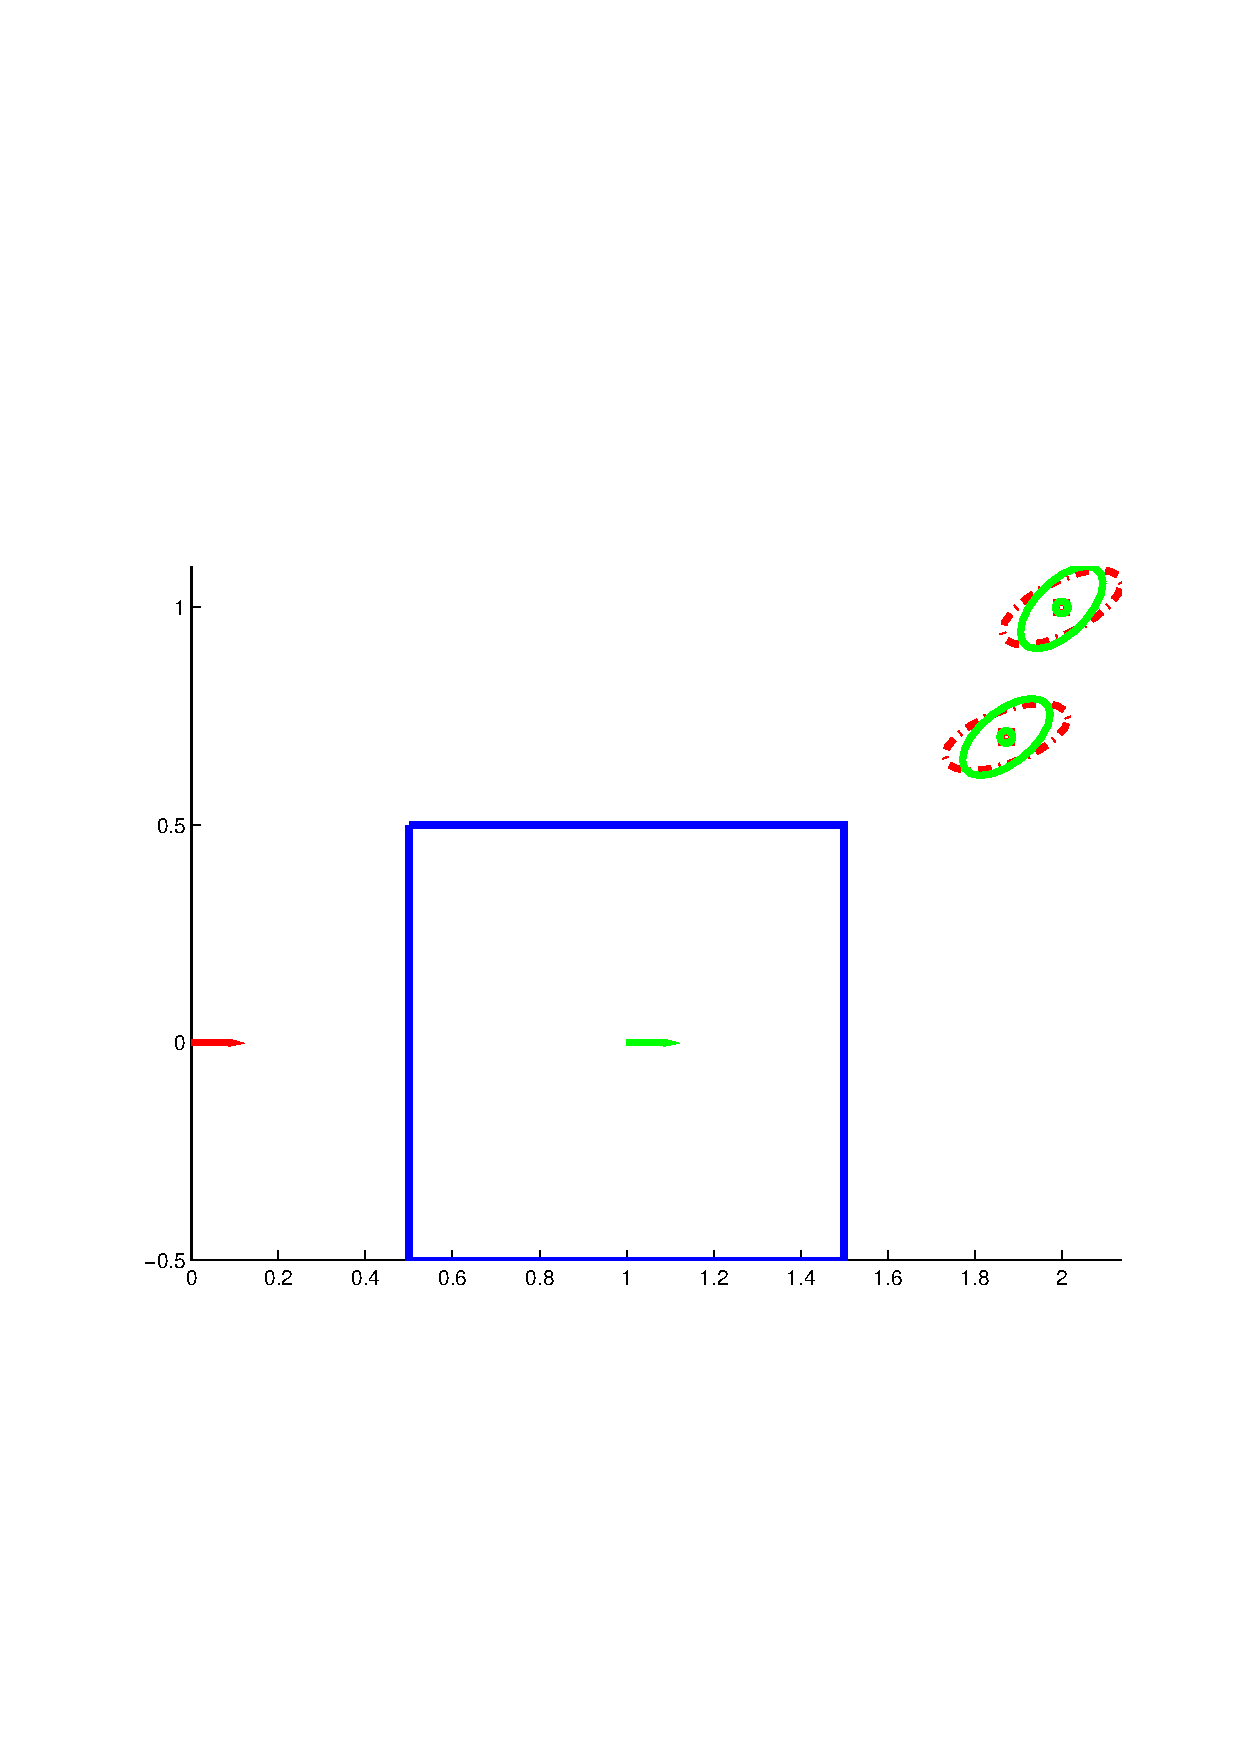
\includegraphics[width=6cm]{Pics/post_example}
\label{fig:post_example}
}
\subfigure[$p({\bf x} | {\bf u})$]{
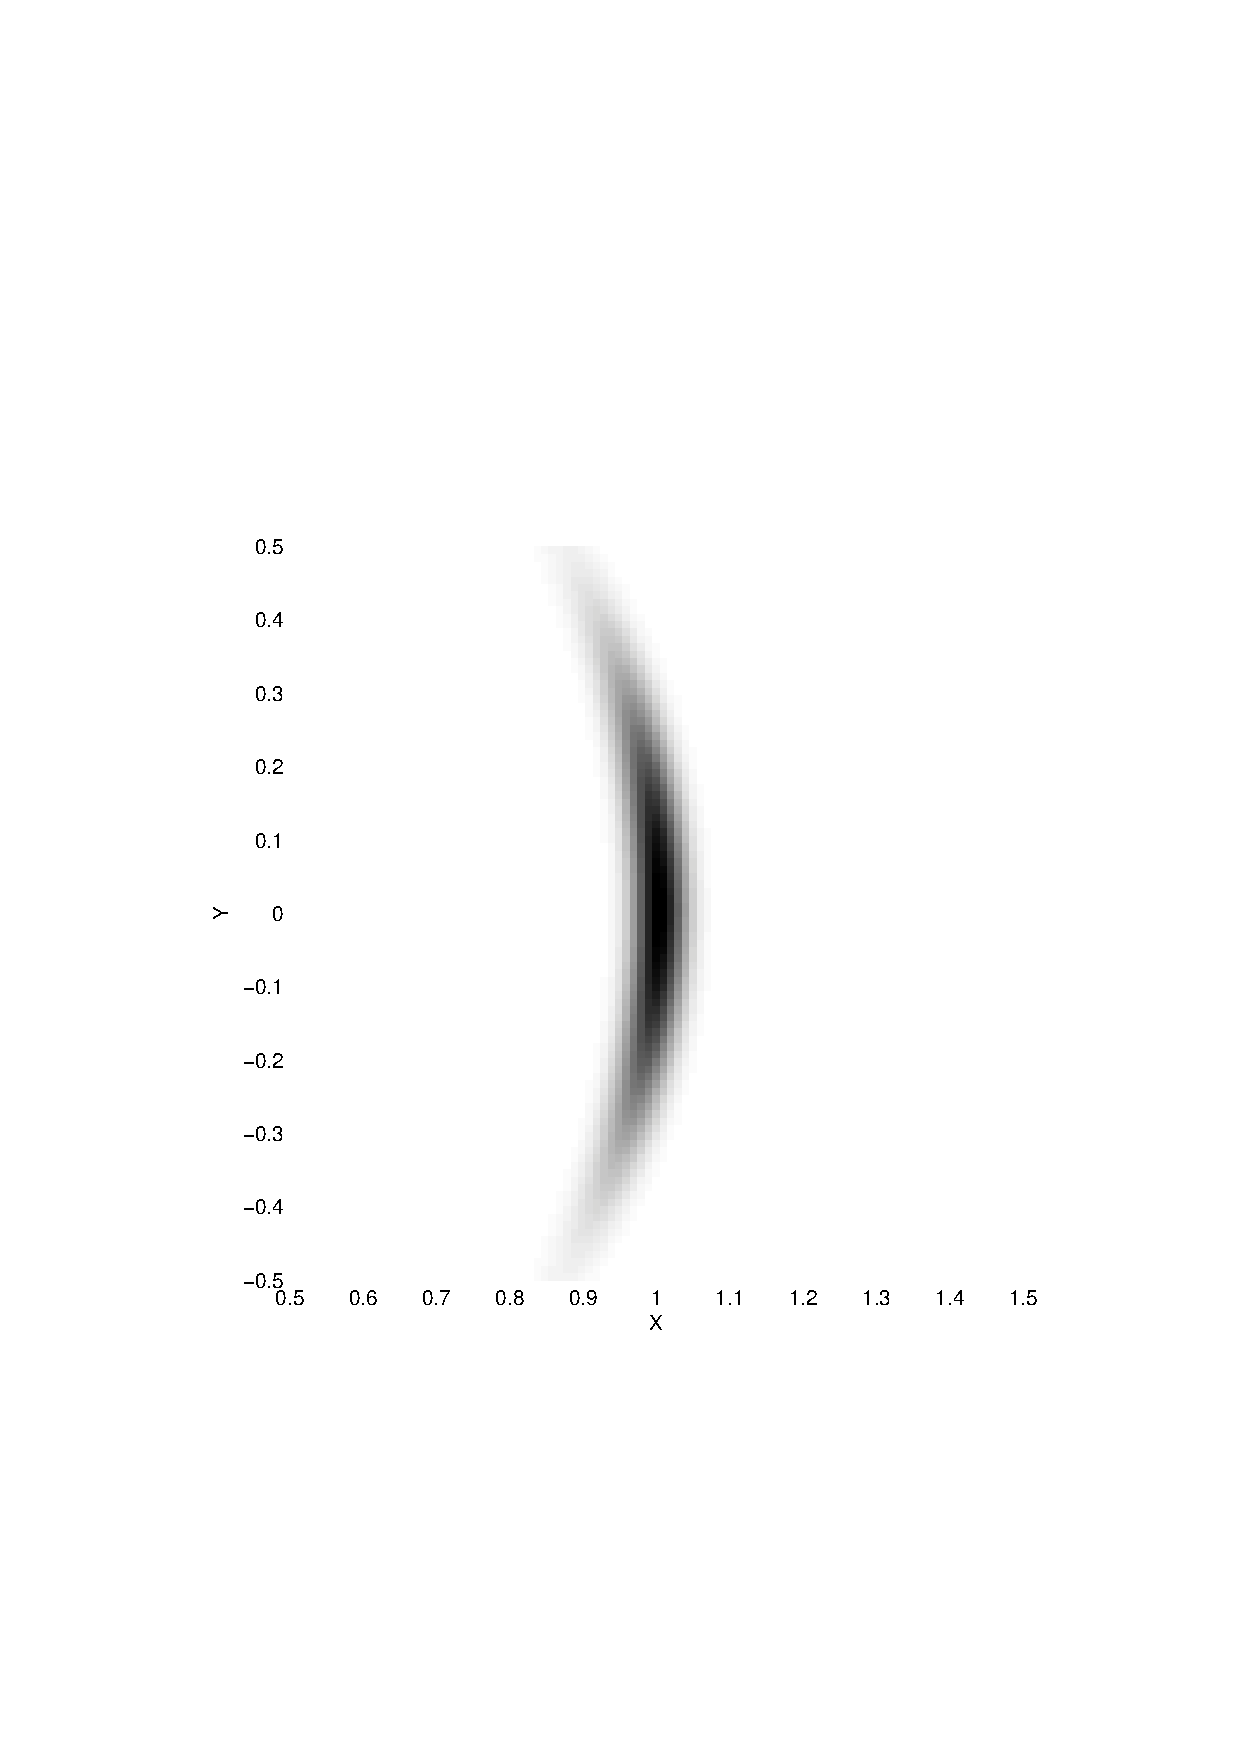
\includegraphics[width=6cm]{Pics/post_odo}
\label{fig:post_odo}
}\\
\subfigure[$p({\bf x} | {\bf z})$]{
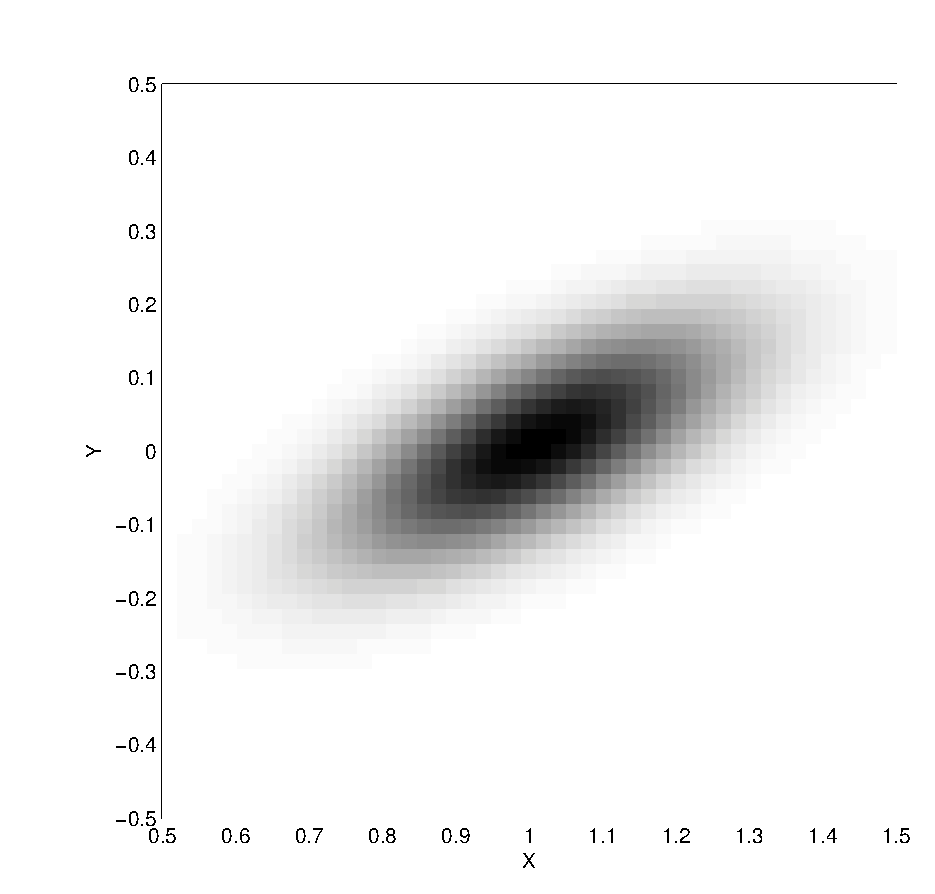
\includegraphics[width=6cm]{Pics/post_obs}
\label{fig:post_obs}
}\quad\space
\subfigure[$p({\bf x} | {\bf u},{\bf z})$]{
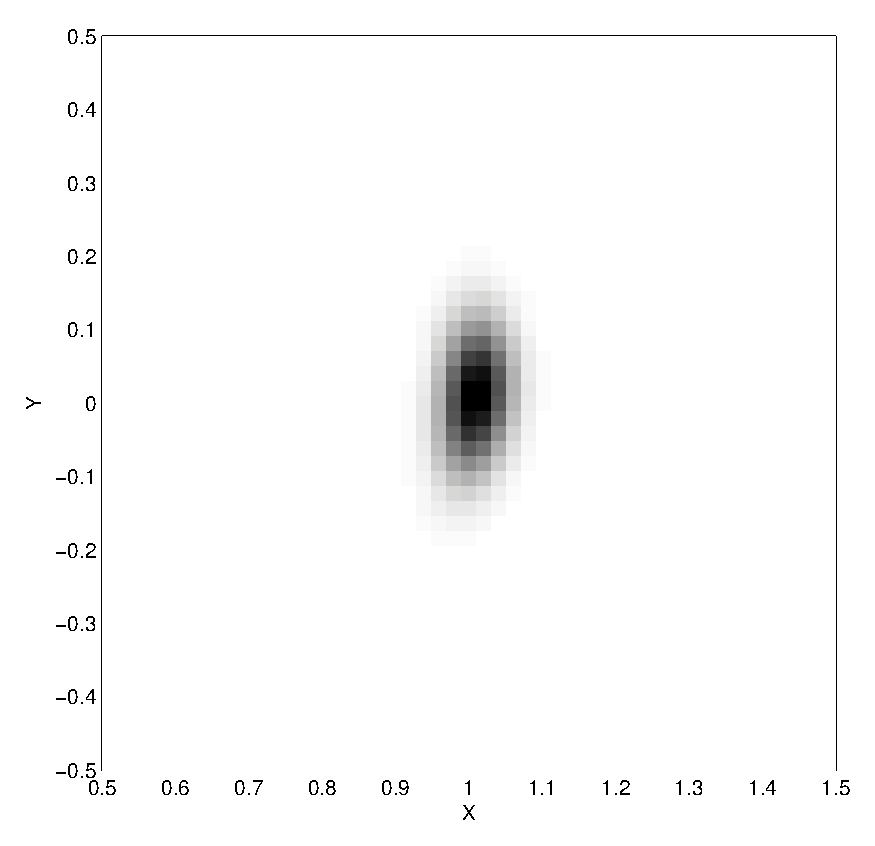
\includegraphics[width=6cm]{Pics/post_obsodo}
\label{fig:post_obsodo}
}
\end{center}
\caption[Robot pose uncertainty, example]
{In \ref{fig:post_example} robot makes observation at point (0,0),
then moves 1 meter forward and makes another observation. The square
shows the region for which pose uncertainty was computed. The
resulting uncertainty just before second measurement is shown in
\ref{fig:post_odo}, the uncertainty due to the measurement is
\ref{fig:post_obs}, and the robot's uncertainty after incorporating
the measurement is \ref{fig:post_obsodo}.}
\label{fig:post_all}
\end{figure}

The main limitation of the EKF approach is the assumption that
uncertainty can be modelled as a Gaussian distribution. Many real life
systems are non-linear, as a result even purely Gaussian noise in
actuation or observation will result in a non-Gaussian posterior
distribution.  

TODO: change example figure to include two uncertainty peaks (data
association uncertainty). 

\refFigure{fig:post_all} illustrates uncertainties involved in the 
robotic mapping system. The robot makes an observation at point (0,0),
then moves one meter forward and makes another observation at
approximately (1,0), see \refFigure{fig:post_example}. The environment
consists of just two landmarks at (2,0.5) and (2,1). We assume they
are distinct, so the robot knows the correspondences between the two
observations. The robot motion is a stochastic process, hence the
robot pose is not known exactly after the execution of the motion
command (in this case move forward 1 meter). The typical resulting
uncertainty for a robot with differential drive system is shown in
\refFigure{fig:post_odo}. As can be seen from the plot  this 
distribution is anything but Gaussian. The ``banana shape'' comes from
the fact that robot is uncertain about the direction of travel, as
well as the distance travelled. Even though the uncertainty about
the distance and direction is zero mean Gaussian, the effect this
uncertainty has on the pose of the robot is far from Gaussian.

\begin{figure}
\begin{center}
\subfigure[EKF ($1\sigma$)]{
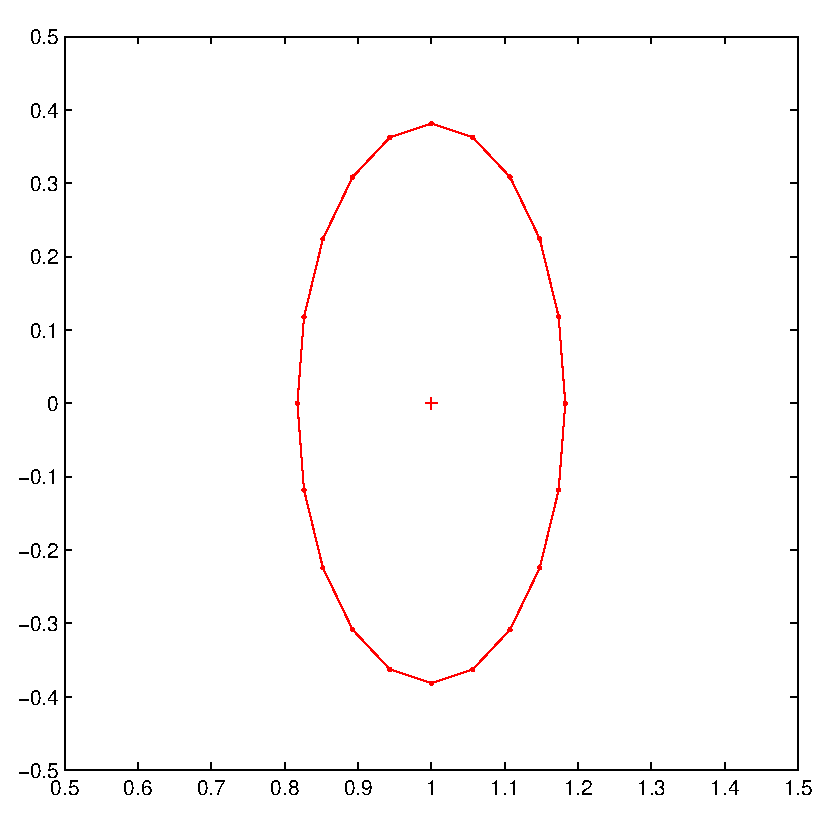
\includegraphics[width=6cm]{Pics/post_odo_ekf}
\label{fig:post_odo_ekf}
}\quad
\subfigure[Particle Filter]{
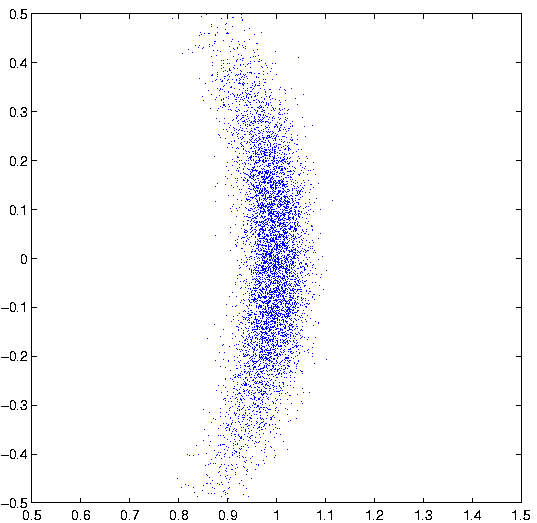
\includegraphics[width=6cm]{Pics/post_odo_pf}
\label{fig:post_odo_pf}
}
\end{center}

\caption[Comparison of uncertainty representation.]
{Modelling of the robot pose uncertainty,
 using EKF (a) and the particle filter (b).
}
\label{fig:post_ekf_vs_pf}
\end{figure}


After execution of the motion command the robot observes the landmarks
once more. Since the observations were not certain for both first and
second observation, the pose estimate that can be derived from the
measurements has a significant uncertainty. This is illustrated in
\refFigure{fig:post_obs}. The posterior distribution is non-Gaussian
in this case as well, although the difference is not as apparent as in
the motion example. The posterior distribution of the robot pose given
observations and control input is shown in
\refFigure{fig:post_obsodo}, and it is obviously non-Gaussian.
\refFigure{fig:post_ekf_vs_pf} illustrates the resulting uncertainty
computed by the EKF and particle filter algorithms after applying a
control input, as in example in \refFigure{fig:post_all}. One can see
that particle filtering captures the banana shape of the motion model
much better than the EKF.


\section{Loop Closing}
\label{sec:back_loop}
%Problem definition
  % Detect
  % Correct

The problem of loop closing arises when mapping a large cyclic
environment. When the robot returns to a previously mapped region via
a large loop, rather than by back-tracing its own steps, it needs to
recognise the place as previously mapped. Failure to do so will result
in incosistent map.  As the robot moves through an unexplored
environment while building the map, it becomes more and more uncertain
about its pose relative to the regions it mapped in the past.
Increased uncertainty of the robot pose makes it more difficult to
detect the place the robot has already mapped.

%The increase in the uncertainty makes it hard for the robot to detect when it comes
%back to the region it has mapped already. 
%Failure to detect revisiting results in an inconsistent map.

In order to build a consistent map, the robot needs to be able to
detect the places it has been to before and correct its estimate of
the path along the loop. The problem of mapping large cyclic
environments has been addressed by several researchers.


%what is there now
  %Lu Milios (scan matching + optimisation)
  %Gutman   (scan matching + confirm + handles high uncertainty)
  %Thrun's  (EM)
  %Fergusson (EKF mines)
  %Atlas


Lu and Milios \cite{lu97:_global} propose an algorithm they call
``consistent pose estimation''. The algorithm uses laser scan matching
and linearised global optimisation over scan poses to build a scan map
of the environment in a single global frame. The approach builds a
network of robot poses at which a laser scan has been taken. The poses
are connected by ``weak'' and ``strong'' links. The links represent
the spatial relations between poses. Weak links are derived from
odometry, and strong links are derived from the scan matches. The
algorithm then finds a global configuration of the poses of the places
by minimising a cost function. If one thinks of links as springs, the
algorithm finds the configuration that reduces the sum of forces
exerted by the springs. Spatial relations are modelled by Gaussians,
and the cost function is the sum of the Mahalanobis distances.

The method by Lu and Milios is very sensitive to the initial estimate
of the robot pose just before loop closing. Since the pose estimate is
derived from the local scan matching and odometry, it can, in
principle, have unbounded error. If the initial estimate is too far
from the real robot pose, the algorithm often converges to local
minima that are not correct. Another problem with this method is the
computational complexity, which is $O(N^3)$ in the number of poses.

Konolige and Gutman
\cite{konolige99:_increm_mappin_large_cyclic_envir} provide a method
based on the ideas of Lu and Milios, but try to address these
problems. Instead of using single laser scan to find relations between
places they use a map correlation technique \cite{konolige99}. This
makes the system more robust to false correspondences. After detecting
loop closing, the algorithm runs consistent pose estimation. 

Another interesting scan matching based mapping technique is
\cite{fergusson2003} by Ferguson \etal. In this approach loop closing
can be undone if the observations further down the track do not
support it.

Thrun \etal \cite{slam_thrun98b,Thrun98a,thrun98:_probab} suggest an
approach that uses an Expectation Maximisation (EM) algorithm for
constructing maps of cyclic environments. The algorithm is given a
relatively small set of observations of sparsely positioned non-unique
landmarks and a set of all control inputs. In the expectation step the
algorithm computes the most likely robot path given the map and the
data. In the maximisation step the most likely map is computed, given
the robots path from the E-step. The Expectation and Maximisation
steps are repeated until the map converges to the maximum likelihood
solution. This algorithm cannot be implemented in real-time, because
it needs to have access to all of the future and past data to
determine the robot pose at any given time.

All of the methods presented so far build a map of the whole
environment in a single global reference frame. Recently, Bosse \etal\
\cite{bosse03atlas} suggest a mapping approach, \Atlas, that does not
require a global reference frame. The map structure used in this
approach is a hybrid topological/metric map.  Each node is a local map
and every link in the topological map represents a spatial
relationship between the two places it connects.  Spatial
relationships are derived from the residual robot pose uncertainty of
the mapping process used to build the local maps. \Atlas\ supports variuos 
underlying mapping modules the two EKF SLAM with line and point features extracted from
either laser or sonar range data. The uncertainty in spatial
relationships are modelled as Gaussians.

\Atlas\ uses a combination of map matching and uncertainty projection
to detect when the robot re-enters a previously explored
area. Uncertainty projection computes the relative poses between the
two non-adjacent local maps. If according to this estimate, the two
maps might be overlapping, \Atlas\ tries to find the landmark
correspondences between the two maps. If the two maps match, the new
link is added to the topological map. The pose relation for this link
is computed from the landmark correspondences. \Atlas\ does not
attempt to correct spatial relations between the map frames along the
closed loop. In order to decrease the probability of incorrect data
association, \Atlas\ runs several hypotheses at any given time. If,
after closing the loop, the observations do not match the map well
enough, the loop closing hypothesis will be discarded in favour of the
new map hypothesis.

The main advantage of \Atlas\ is the map structure it uses. Moving
away from the single reference frame allows the mapping of large
environments with huge cycles in real time. There are some
deficiencies in their approach though. For instance, when the robot
returns to the previously mapped region it gains new knowledge about
relative positions of the local maps. The robot can use this knowledge
to update the links in the map. \Atlas\ does not perform this update
because of the computational requirements involved, although the
authors mention that such update can be performed after the mapping is
complete. \Atlas\ uses metrics to test loop closing hypotheses. These
metrics do not necessarily correspond to the true likelihood, making
it difficult to predict the behaviour of the algorithm in a new
environment. 

\SILENT{how do you tune these metrics if you have a different sensor,
  than what they used?}

\section{Summary}

The past few decades of mobile robotics research provide us with
the tools for mapping and localisation. Unfortunately, existing
algorithms work only in relatively small environments. The main
limiting factors are:

\begin{itemize}
\item The computational burden: as size of the environment grows, so do
  the computational requirements of existing algorithms.

\item The data association problem in the face of uncertainty: 
   in large environments the uncertainty of the landmarks far away
  from the origin is high. That makes it difficult to perform correct
  data association.

\end{itemize}

Various optimisation techniques and faster hardware can expand the
capabilities of existing algorithms, but to really overcome these
limitations new map representations are required. In particular new
ways to model uncertainty should be explored. Some recent research in
this area include \cite{bosse03atlas,fergusson2003}.

% LocalWords:  Kalman odometry EKF FastSLAM Bayes MCL Lu Milios Konolige Gutman
% LocalWords:  Thrun Bosse Ferguson resampling Gaussians linearisation
